% questions.tex —— 1987 年·上海卷·数学 · 题目内容片段（无答案）
% 由 tools/generate_projects.py 依来源总账自 1987/1987_数学真题_上海_试题.md 生成，勿手改（改源 MD 后重跑）


\begin{gktip}
\textbf{来源说明}：本题面依据固定源 PDF《1987 年上海市普通高等学校招生统一考试数学试题》逐题转录。固定源共 3 页，PDF 无可用文字层，题面和答案与略解均在同一文件内；下列题面以高清渲染图为依据。

\textbf{图形说明}：第 2 题的四个函数图象选项和第 4 题的三棱锥图依据固定源图形关系重绘为 TikZ 矢量图。
\end{gktip}

\begin{question}
\gkti{1}

第一题（本题满分 36 分）共有 12 个小题，只要求直接填写结果，填对得 3 分，否则一律得 0 分。

（1） $y=x^3\ (x\leq0)$ 的反函数是 $\underline{\hspace{4em}}$。

\Needspace{5\baselineskip}
（2） 计算下式：

\nopagebreak[4]
\[
C_{10}^{1}+C_{10}^{2}+\cdots+C_{10}^{9}+C_{10}^{10}
\]

的值是 $\underline{\hspace{4em}}$。

\Needspace{5\baselineskip}
（3） 函数

\nopagebreak[4]
\[
f(x)=ax^2+bx+c
\]

是偶函数的充要条件是 $\underline{\hspace{4em}}$。

（4） 设 $ABCD-A_1B_1C_1D_1$ 为一正方体，$E,F$ 分别为 $BB_1,DC_1$ 的中点，则 $AE$ 与 $D_1F$ 所成的角为 $\underline{\hspace{4em}}$。

（5） 在底面半径为 $a$、高为 $2a$ 的圆柱中，分别挖去一个底面半径及高均为 $a$ 的圆锥与一个半径为 $a$ 的半球，则剩下部分的体积为 $\underline{\hspace{5em}}$。

\Needspace{5\baselineskip}
（6） 函数

\nopagebreak[4]
\[
y=2\left|\sin\left(4x-\frac\pi3\right)\right|
\]

的最小正周期为 $\underline{\hspace{4em}}$。

\Needspace{5\baselineskip}
（7） 计算函数值：

\nopagebreak[4]
\[
\arcsin\left(\sin\frac{3\pi}{5}\right)=\underline{\hspace{4em}}.
\]

\Needspace{5\baselineskip}
（8） 双曲线

\nopagebreak[4]
\[
4x^2-(y-3)^2=4
\]

的渐近线方程为 $\underline{\hspace{8em}}$。

\Needspace{5\baselineskip}
（9） 由参数方程

\nopagebreak[4]
\[
x=2(\sec^2\theta-1),\qquad y=2\operatorname{tg}\theta,
\qquad -\frac\pi2<\theta<\frac\pi2
\]

给出的曲线在直角坐标系下的方程为 $\underline{\hspace{6em}}$。

（10） 设 $\{a_n\}$ 为等差数列，已知 $a_1=1$，$a_5$ 与 $a_9$ 的算术平均数为 $19$，则该等差数列的公差为 $\underline{\hspace{4em}}$。

（11） $\left(x-\dfrac1x\right)^8$ 的展开式中，$x^4$ 的系数与 $\dfrac1{x^4}$ 的系数之差是 $\underline{\hspace{4em}}$。

\Needspace{5\baselineskip}
（12） 设 $2^a=5^b=10$，则

\nopagebreak[4]
\[
\frac1a+\frac1b=\underline{\hspace{4em}}.
\]

\Needspace{0.4\textheight}
\end{question}
\begin{question}
\gkti{2}

第二题（本题满分 36 分）共有 12 个小题，每题都给出代号为 A、B、C、D 的四个结论，其中有一个结论是正确的；选对得 3 分，不选、选错或选出的代号超过一个，一律得 0 分。

\Needspace{5\baselineskip}
（1） 设函数

\nopagebreak[4]
\[
y=\log_2x+3\qquad(x\geq1),
\]

则 $y$ 的值域是\mbox{（　　）}

（A）$\{y\mid y\geq3\}$　　（B）$\{y\mid y>3\}$

（C）$\{y\mid y\geq5\}$　　（D）$R$

（2） 下列函数图象中，表示 $y=x^{\frac23}$ 的是\mbox{（　　）}
\nopagebreak[4]
\begin{center}% 1987 年上海卷第二题：y=x^(2/3) 的四个图象选项
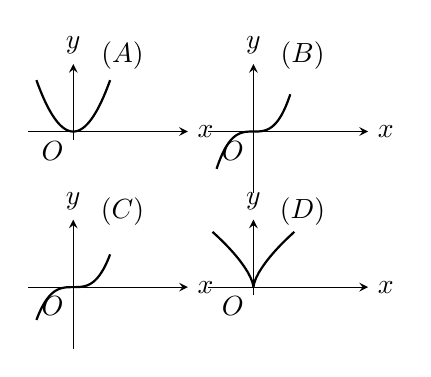
\begin{tikzpicture}[scale=0.52,>=stealth]
  \node at (1.2,1.85) {$(A)$};
  \draw[->] (-1.1,0)--(2.8,0) node[right] {$x$};
  \draw[->] (0,-0.2)--(0,1.65) node[above] {$y$};
  \draw[thick,domain=-0.9:0.9,samples=80] plot (\x,{1.55*\x*\x});
  \node[below left] at (0,0) {$O$};

  \begin{scope}[xshift=4.4cm]
    \node at (1.2,1.85) {$(B)$};
    \draw[->] (-1.1,0)--(2.8,0) node[right] {$x$};
    \draw[->] (0,-1.5)--(0,1.65) node[above] {$y$};
    \draw[thick,domain=-0.9:0.9,samples=80] plot (\x,{1.25*\x*\x*\x});
    \node[below left] at (0,0) {$O$};
  \end{scope}

  \begin{scope}[yshift=-3.8cm]
    \node at (1.2,1.85) {$(C)$};
    \draw[->] (-1.1,0)--(2.8,0) node[right] {$x$};
    \draw[->] (0,-1.5)--(0,1.65) node[above] {$y$};
    \draw[thick,domain=-0.9:0.9,samples=80] plot (\x,{1.1*\x*\x*\x});
    \node[below left] at (0,0) {$O$};
  \end{scope}

  \begin{scope}[xshift=4.4cm,yshift=-3.8cm]
    \node at (1.2,1.85) {$(D)$};
    \draw[->] (-1.1,0)--(2.8,0) node[right] {$x$};
    \draw[->] (0,-0.2)--(0,1.65) node[above] {$y$};
    \draw[thick,domain=-1.0:0,samples=80] plot (\x,{1.35*abs(\x)^(2/3)});
    \draw[thick,domain=0:1.0,samples=80] plot (\x,{1.35*abs(\x)^(2/3)});
    \node[below left] at (0,0) {$O$};
  \end{scope}
\end{tikzpicture}
\end{center}
\nopagebreak[4]
（3） 设实数 $a,b$ 满足 $0<a<b$ 且 $a+b=1$，则下列四数中最大的是\mbox{（　　）}

（A）$\dfrac12$　　（B）$a^2+b^2$　　（C）$2ab$　　（D）$a$

（4） 设 $0<\theta<45^\circ$，则 $\cos^2\theta,\sin^2\theta,\operatorname{ctg}^2\theta$ 的大小规律是\mbox{（　　）}

（A）$\cos^2\theta<\sin^2\theta<\operatorname{ctg}^2\theta$

（B）$\operatorname{ctg}^2\theta<\sin^2\theta<\cos^2\theta$

（C）$\sin^2\theta<\cos^2\theta<\operatorname{ctg}^2\theta$

（D）$\cos^2\theta<\operatorname{ctg}^2\theta<\sin^2\theta$

\Needspace{5\baselineskip}
（5） 计算下式：

\nopagebreak[4]
\[
\frac{\sin\alpha+\sin\beta}{\cos\alpha+\cos\beta}
\]

等于\mbox{（　　）}

（A）$\operatorname{tg}\dfrac{\alpha+\beta}{2}$　　（B）$-\operatorname{tg}\dfrac{\alpha+\beta}{2}$

（C）$\operatorname{tg}\alpha+\operatorname{tg}\beta$　　（D）$\operatorname{ctg}\dfrac{\alpha+\beta}{2}$

\Needspace{5\baselineskip}
（6） 如果圆

\nopagebreak[4]
\[
x^2+y^2+ax+by+c=0\qquad(a,b,c\text{ \text{不全为} }0)
\]

与 $x$ 轴相切于原点，那么\mbox{（　　）}

（A）$a=0,\ b\ne0,\ c\ne0$　　（B）$b=c=0,\ a\ne0$

（C）$a=c=0,\ b\ne0$　　（D）$a=b=0,\ c\ne0$

（7） 直线 $x+2y+3=0$ 的倾斜角为\mbox{（　　）}

（A）$\operatorname{arctg}\left(-\dfrac12\right)$　　（B）$\operatorname{arctg}\dfrac12$

（C）$\dfrac\pi2+\operatorname{arctg}\dfrac12$　　（D）$\pi-\operatorname{arctg}\dfrac12$

\Needspace{5\baselineskip}
（8） 极坐标方程

\nopagebreak[4]
\[
\rho=\frac6{3+2\sin\left(\frac32\pi+\theta\right)}
\]

所表示的图形是\mbox{（　　）}

（A）圆　　（B）椭圆　　（C）双曲线　　（D）抛物线

（9） 在空间里，下述命题中正确的是\mbox{（　　）}

（A）若直线 $a\parallel$ 平面 $M$，直线 $b\perp$ 直线 $a$，则直线 $b\perp$ 平面 $M$。

（B）若平面 $M\parallel$ 平面 $N$，则平面 $M$ 内任意一条直线 $a\parallel$ 平面 $N$。

（C）若平面 $M$ 与平面 $N$ 的交线为 $a$，平面 $M$ 内的直线 $b\perp$ 直线 $a$，则直线 $b\perp$ 平面 $N$。

（D）若平面 $N$ 内的两条直线都平行于平面 $M$，则平面 $N\parallel$ 平面 $M$。

（10） 三个互不重合的平面能把空间分成 $n$ 个部分，$n$ 的所有可能值为\mbox{（　　）}

（A）$4,6,7$　　（B）$4,5,6,8$　　（C）$4,7,8$　　（D）$4,6,7,8$

\Needspace{5\baselineskip}
（11） 若直线

\nopagebreak[4]
\[
l_1:ax+2y+6=0
\]

\Needspace{5\baselineskip}
与直线

\nopagebreak[4]
\[
l_2:x+(a-1)y+(a^2-1)=0
\]

平行但不重合，则 $a$ 等于\mbox{（　　）}

（A）$-1$ 或 $2$　　（B）$-1$　　（C）$2$　　（D）$\dfrac23$

（12） 七人并排成一行，如果甲、乙两人必须不相邻，那么不同排法的种数是\mbox{（　　）}

（A）1440　　（B）3600　　（C）4320　　（D）4800

\end{question}
\begin{question}
\gkti{3}

\Needspace{5\baselineskip}
第三题（本题满分 7 分）。设

\nopagebreak[4]
\[
A=\left\{x\middle|\log_{\frac13}\left|x-\frac\pi3\right|
\geq\log_{\frac13}\frac{2\pi}{3},\ x\in R\right\},
\]

\nopagebreak[4]
\[
B=\{x\mid\cos x\geq0,\ x\in R\}.
\]

求 $D=A\cap B$，最后结果用区间形式表示，并在数轴上标出符合 $D$ 的部分。

\Needspace{0.4\textheight}
\end{question}
\begin{question}
\gkti{4}

\Needspace{5\baselineskip}
第四题（本题满分 8 分）共有 3 个小题。设三棱锥 $S-ABC$ 的底面为等腰直角三角形，已知该直角三角形的斜边 $AC$ 长为 $10$，三棱锥的侧棱

\nopagebreak[4]
\[
SA=SB=SC=13.
\]

（1） 顶点 $S$ 到底面的距离；

（2） 侧棱 $SB$ 与底面所成角的大小（用反三角函数表示）；

（3） 二面角 $A-SB-C$ 的大小（用反三角函数表示）。
\nopagebreak[4]
\begin{center}% 1987 年上海卷第四题：三棱锥 S-ABC
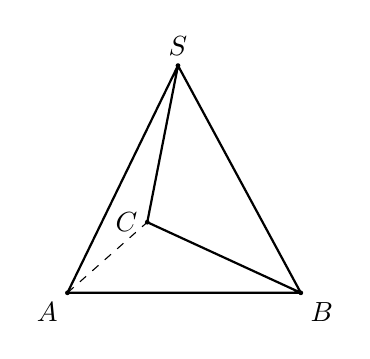
\begin{tikzpicture}[scale=0.78,>=stealth]
  \coordinate (S) at (1.8,3.7);
  \coordinate (A) at (0,0);
  \coordinate (B) at (3.8,0);
  \coordinate (C) at (1.3,1.15);
  \draw[thick] (S)--(A) (S)--(B) (S)--(C) (A)--(B) (B)--(C);
  \draw[dashed] (A)--(C);
  \fill (S) circle (1.1pt) node[above] {$S$};
  \fill (A) circle (1.1pt) node[below left] {$A$};
  \fill (B) circle (1.1pt) node[below right] {$B$};
  \fill (C) circle (1.1pt) node[left] {$C$};
\end{tikzpicture}
\end{center}
\nopagebreak[4]
\end{question}
\begin{question}
\gkti{5}

\Needspace{5\baselineskip}
第五题（本题满分 9 分）。设 $A(x_1,y_1)$ 为椭圆

\nopagebreak[4]
\[
x^2+2y^2=2
\]

\Needspace{5\baselineskip}
上的任意一点，过点 $A$ 作一条斜率为

\nopagebreak[4]
\[
-\frac{x_1}{2y_1}
\]

\Needspace{5\baselineskip}
的直线 $l$，又设 $d$ 为原点到直线 $l$ 的距离，$r_1,r_2$ 分别为点 $A$ 到椭圆两个焦点的距离。试证明

\nopagebreak[4]
\[
\sqrt{r_1r_2}\cdot d
\]

为常数。

\end{question}
\begin{question}
\gkti{6}

第六题（本题满分 12 分）本题共有 2 个小题，第 1 小题满分 5 分，第 2 小题满分 7 分。

\Needspace{5\baselineskip}
在 $xOy$ 平面上给定一曲线

\nopagebreak[4]
\[
y^2=2x.
\]

（1） 设点 $A$ 的坐标为 $\left(\frac23,0\right)$，求曲线上距点 $A$ 最近的点 $P$ 之坐标及相应的距离 $|PA|$；

（2） 设点 $A$ 的坐标为 $(a,0)$，$a\in R$，求曲线上点距点 $A$ 的距离之最小值，并写出 $d=f(a)$ 的函数表达式。

\end{question}
\begin{question}
\gkti{7}

第七题（本题满分 12 分）本题共有 3 个小题，第 1 小题满分 4 分，第 2 小题满分 5 分，第 3 小题满分 3 分。

设复平面上有一系列向量 $\overrightarrow{OZ_n}$（$n=0,1,2,\ldots$）满足如下关系：将 $\overrightarrow{OZ_n}$ 逆时针方向旋转 $\frac34\pi$ 后，再把它的模变为原来的一半，得到 $\overrightarrow{OZ_{n+1}}$。记 $\overrightarrow{OZ_n}$ 所对应的复数为 $z_n$（$n=0,1,2,\ldots$）。

\Needspace{5\baselineskip}
若

\nopagebreak[4]
\[
z_0=2\sqrt2+2\sqrt2\,i,
\]

且复数的辐角为辐角的主值，

（1） 求 $z_n$；

（2） $n$ 为何值时，$z_n$ 为实数？将所有等于实数的 $z_n$ 按原有次序排成数列 $\{a_n\}$，写出该数列的通项公式；

\Needspace{5\baselineskip}
（3） 求

\nopagebreak[4]
\[
\lim_{k\to\infty}(a_1+a_2+\cdots+a_k).
\]

\end{question}